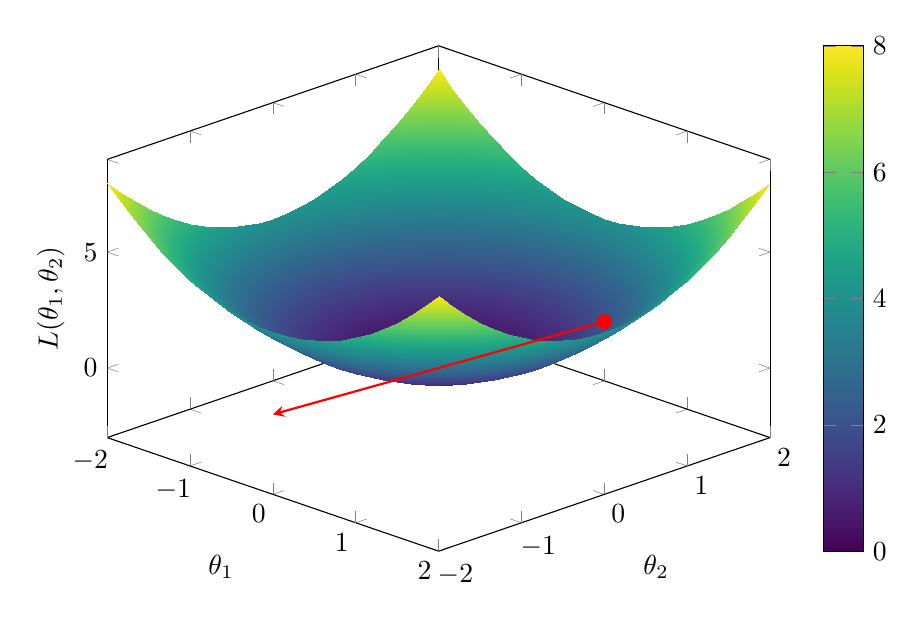
\begin{tikzpicture}
    \begin{axis}[
        width=10cm,
        height=8cm,
        view={45}{30},
        xlabel={$\theta_1$},
        ylabel={$\theta_2$},
        zlabel={$L(\theta_1,\theta_2)$},
        domain=-2:2,
        y domain=-2:2,
        colormap/viridis,
        colorbar,
    ]
    % 绘制损失函数曲面
    \addplot3[
        surf,
        shader=interp,
    ] {x^2 + y^2};
    
    % 标记一个具体点 (1,1)
    \addplot3[
        only marks,
        mark=*,
        mark options={fill=red},
        red,
        mark size=2.5pt,
    ] coordinates {(1,1,{1^2+1^2})};
    
    % 绘制负梯度向量(在点 (1,1)处计算)
    % 由于梯度为 (2*1, 2*1),负梯度为 (-2, -2)。
    % 为了在三维图中展示,我们对z方向也给定一个缩放因子,便于直观展示。
    \addplot3[
        -stealth,
        red,
        thick,
        quiver={
            u={-2},
            v={-2},
            w={-0.5*(2^2+2^2)}  % 此处w分量用于调整图示效果
        },
        domain=0:0.5,
        samples=2,
    ] coordinates {(1,1,{1^2+1^2})};
    \end{axis}
    \end{tikzpicture}
    